\noindent \textcolor{myBlue}{\textbf{\large{3 DESENVOLVIMENTO }}}\\

\noindent \textbf{Projeto proposto:} tendo as seguintes espificações: mf = $45^o$ mg = $12$ dB e $e_{ss} = 0,01$. 

\begin{figure}[H]
\centering
\begin{tikzpicture}

\sbEntree{E}
\sbComp{comp}{E}
\sbRelier[$R(s)$]{E}{comp}
\sbBloc{B}{$K$}{comp}
\sbRelier{comp}{B}
\sbBloc{C}{$G(s)$}{B}
\sbRelier{B}{C}
\sbSortie[4]{S}{C}
\sbRelier{C}{S}
\sbNomLien[0.8]{S}{$C(s)$} \sbRenvoi{C-S}{comp}{}

\end{tikzpicture}
\end{figure}

\noindent Determine o compensador de avanço para a planta:

\[ G(s) = \dfrac{10}{s\cdot (s+15)}\]

\noindent \textbf{Solução:} \\

\noindent \textbf{1. Definir o numero do tipo da função de transferência da planta:} \\

Tem-se por definição que o tipo da função se dá pelo numero de polos na origem, no casa da função $G(s)$, existe 2 polos $s_1 = 0$ e $s_2 = -15$. Logo, temos apenas um polo na origem {\color{red}a função de transferência da planta é do tipo 1}.

No Matlab a função da planta foi definida como $G$, tendo em vista sua forma simplificada:

\[G(s) = \dfrac{10}{s^2 + 15s}\]

\noindent Segue o código: 

\begin{lstlisting}[style=matlab]
nump = 10;
denp = [1 15 0];
G = tf(nump,denp)
\end{lstlisting}\vspace{0.2cm}

%%%%%%%%%%%%%%%%%%%%%%%%%%%%%%
%             PARTE 2
%%%%%%%%%%%%%%%%%%%%%%%%%%%%%%


\noindent \textbf{2. Calcular o ganho adicional $K_c$ necessário para atender o requisito de precisão ($e_{ss}$ – erro estático):} \\

Por definição temos que para o tipo 1 de função de transferência:

\begin{center}
\( e_{ss} = \dfrac{1}{K_v} \), onde \( K_v = \lim_{s \to 0} s\cdot G(s) \)
\end{center}

sendo assim, podemos calcular o $K_v$ atual,

\[ K_v = \lim_{s \to 0} s \dfrac{10}{s\cdot(s+15)} \Rightarrow K_v = \lim_{ s \to 0} \dfrac{10}{(0+15)} = \dfrac{10}{15}\]

com isso podemos supor a adição de um controlador, que será chamado de $C(s)$, tendo em vista que o erro especificado para o projeto é de $0,01$, podemos achar o novo $K_v$, \newpage

\[e_{ss} = 0,01 = \dfrac{1}{K_v} \Rightarrow K_v = 100\]

logo, considerando a equação para nosso compensador sendo,

\[ C(s) = K_c \cdot \dfrac{Ts + 1}{\alpha T s + 1} \]

nossa planta compensada terá forma $C(s)G(s)$, com isso se pode calcular o valor do ganho adicional necessário $K_c$,

\[K_{v} = 100 = \lim_{^s \to 0} s \cdot K_c \cdot \dfrac{Ts + 1}{\alpha T s + 1} \cdot \dfrac{10}{s(s+15)} \Rightarrow \lim_{s \to 0} K_c \cdot \dfrac{10}{(0+15)}\cdot \dfrac{T\cdot 0 + 1}{\alpha T \cdot 0 + 1} = 100 \]

\[ K_c \cdot \dfrac{10}{15} = 100\]

{\color{red}
	\[\boxed{K_c = 150}\]
}

Esse será o valor de ganho adicional, será adicionado ao matlab de tal forma:

\begin{lstlisting}[style=matlab]
Kc = 150;
\end{lstlisting}\vspace{0.2cm}



%%%%%%%%%%%%%%%%%%%%%%%%%%%%%%
%             PARTE 3
%%%%%%%%%%%%%%%%%%%%%%%%%%%%%%

\noindent\textbf{3. Calcular a função de transferência G(s) do sistema não compensado, e com o ganho ajustado. Plotar os gráficos logarítmicos de $G(j\omega)$ e obter as margens de fase e de ganho.}\\

Tendo já definido a função $G(s)$ no tópico 1, será feito apenas o plot da mesma seguindo o código:

\begin{lstlisting}[style=matlab]
figure(1)
bode(G)
margin(G)
grid
\end{lstlisting}\vspace{0.2cm}

tal código irá gerar o gráfico da \textbf{Figura 1}, onde encontramos mg = $\infty$ e mf = $87,5^o$, para o sistema não compensado.\\

Agora ajustando a função de transferência com $K_c$, acharemos uma primeira estimativa da frequência de cruzamento, teremos a função $Kc\cdot G(s)$,

\[ Kc\cdot G(s) = 150\cdot \dfrac{10}{s^2+15s} \]


\noindent utilizando o código:

\begin{lstlisting}[style=matlab]
GKc=tf(Kc*nump,denp);
figure(2)
bode(GKc)
margin(GKc)
grid
\end{lstlisting}\vspace{0.2cm}

Com isso encontramos o gráfico da \textbf{Figura 2}, onde temos {\color{red}mf = $21,9$ na frequência $37,3$ rad/s e mf = $\infty$}.

\begin{figure}[H]
  \centering
  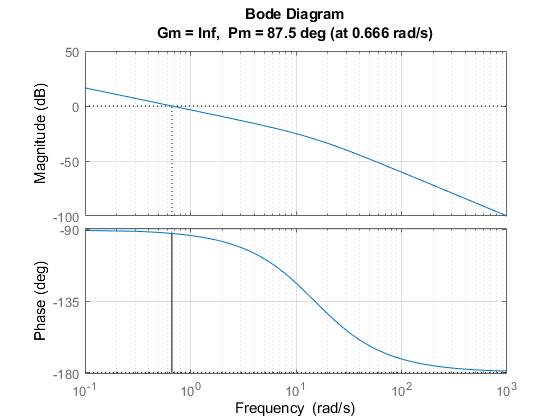
\includegraphics[width=0.8\textwidth]{images/fig1.png}
  \caption{Bode da planta não compensada}
\end{figure}

\begin{figure}[H]
  \centering
  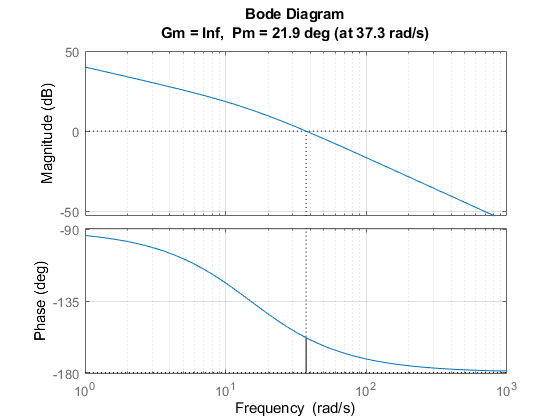
\includegraphics[width=0.8\textwidth]{images/fig2.png}
  \caption{Bode da planta com o ganho compensado}
\end{figure}
\newpage

%%%%%%%%%%%%%%%%%%%%%%%%%%%%%%
%             PARTE 4
%%%%%%%%%%%%%%%%%%%%%%%%%%%%%%

\textbf{4. Calcular a defasagem máxima do compensador por avanço de fase, os parâmetros $\alpha$ e T do compensador.}\\

Como a margem de fase é aproximadamente $21,9^o$ a frequencia em torno de $37,3$ rad/s. Podemos calcular o $\phi_m$ (defasagem máxima), considerando a margem de fase de $45^o$ específicado e somando $5^o$ como folga, por conta de que a frequência de cruzamente será sempre maior pela ação do controlador. Assim teremos, 

\[\phi_m = 45 - 21,9 + 5\]

{\color{red}\[ \boxed{\phi_m = 28,1^o} \]}

Determinando a posição "relativa" do polo em relação ao zero, a razao entre as frequências do zero e do polo, que é igual a $\alpha$, que é dado por,

\[ \alpha = \dfrac{1-sen(\frac{\phi_m \pi}{180})}{1+sen(\frac{\phi_m \pi}{180})} = \dfrac{1-sen(\frac{28,1\pi}{180})}{1+sen(\frac{28,1 \pi}{180})} \]

{\color{red}\[ \boxed{\alpha = 0,3596} \]}

Determinando a "localização" da resposta em frequência do controlador, ou seja, encontrar wm, frequência em que ocorre $\phi_m$. Nessa frequência o ganho do controlador é (em dB):

\[ Gc_{wm}=20log_{10}(Kc\sqrt(\alpha)) = 20log_{10}(\frac{150}{\sqrt{0,3596}}) = 47.96 \]

Para que wm seja a nova frequência de cruzamento, o ganho de malha nessa fequencia deve ser 1. Ou seja, o ganho da planta (sem Kc obviamente) deve ser o inverso do ganho do controlador nessa frequência. Em dB, o ganho da planta deve ser o recíproco (negativo) do ganho do controlador, logo deve ser igual a $-47.96$ dB. Utilizando manualmente um data tip do matlab na \textbf{Figura 1}, podemos encontrar o valor de $\omega_m$:

\begin{figure}[H]
  \centering
  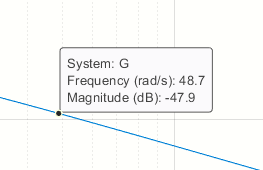
\includegraphics[width=0.5\textwidth]{images/fig3.png}
  \caption{Data tip no primeiro plot para achar $\omega_m$}
\end{figure} \newpage

Nota-se que em torno da fequencia $48,7$ rad/s a planta tem ganho $-Gc_{wm}$ (em dB). Portanto o valor encontrado em 28.3 dB é,

{\color{red} \[ \boxed{\omega_m = 48,7} \]}

Com isso encontramos o último valor, 

\[ T = \dfrac{1}{\omega_m \cdot \sqrt{\alpha}} = \dfrac{1}{48,7\cdot \sqrt{0,3596}}\]

{\color{red} \[ \boxed{T = 0.,0342} \] }

\noindent Em matlab, foi usado os seguintes comandos para realizar tais cálculos:

\begin{lstlisting}[style=matlab]
phi_m=28.1;
a=(1-sin(phi_m*pi/180))/(1+sin(phi_m*pi/180))
Gc_wm=20*log10(Kc/sqrt(a)) 
%olhar grafico 1 com data tip
wm=48.7; 
T=1/(wm*sqrt(a)) 
\end{lstlisting}\vspace{0.2cm}

%%%%%%%%%%%%%%%%%%%%%%%%%%%%%%
%             PARTE 5
%%%%%%%%%%%%%%%%%%%%%%%%%%%%%%

\noindent \textbf{5. Escrever a função de transferência do compensador C(s).}\\

Com os parâmetros encontrados basta substitui-los,

\[ C(s) = K_c \dfrac{Ts+1}{\alpha T s + 1} = 150\dfrac{0,0342s + 1}{0,0342\cdot 0,3596 s + 1}\]

{\color{red} \[ \boxed{C(s) = \dfrac{5.136 s + 150}{0.01231 s + 1} } \]}

\noindent Em matlab:

\begin{lstlisting}[style=matlab]
numc=Kc*[T 1];
denc=[a*T 1];
C=tf(numc,denc)
\end{lstlisting}\vspace{0.2cm}

%%%%%%%%%%%%%%%%%%%%%%%%%%%%%%
%             PARTE 6
%%%%%%%%%%%%%%%%%%%%%%%%%%%%%%

\noindent \textbf{6. Compensar o sistema; desenhar os gráficos logarítmicos do sistema compensado e verificar as margens de fase e de ganho obtidas.}\\

Para isso foi usado o matlab, compensando em uma função de transferência nomeada $CG(s)$ para simplificar o entendimento, segue o cógigo:

\begin{lstlisting}[style=matlab]
CG=C*G;
figure(3)
bode(CG)
margin(CG)
grid
\end{lstlisting}\vspace{0.2cm}

Com isso tivemos o seguinte gráfico da planta do sistema compensado:

\begin{figure}[H]
  \centering
  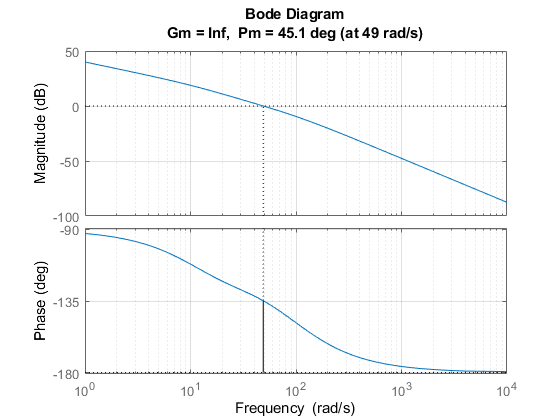
\includegraphics[width=0.8\textwidth]{images/fig4.png}
  \caption{Bode da planta do sistema compensado}
\end{figure}

Com isso encontramos o ganho de fase igual a $45,1^o$, o que fica muito próximo do específicado no projeto.

E a margem de ganho encontrada foi de $\infty$, o que significa que o sistema ficará estável, não importa o quanto for aumentado o ganho.

{\color{red} Logo, o sistema está dentro das especificações do projeto.}\\

%%%%%%%%%%%%%%%%%%%%%%%%%%%%%%
%             PARTE 7
%%%%%%%%%%%%%%%%%%%%%%%%%%%%%%

\noindent \textbf{7. Fechar a malha de controle (realimentação unitária e negativa) e obter o gráfico da resposta transitória.}\\

Para um melhor entendimento, no gráfico foi colado tanto o sistema não compensado quanto o com o controlador. E após foi feito gráfico apenas da resposta do sistema com o controlador.

\noindent Com o seguinte código em matlab:

\begin{lstlisting}[style=matlab]
Y_R=feedback(G,1); % sem controlador!!!
Y_R2=feedback(CG,1);  % com controlador

figure(4)
step(Y_R,'b',Y_R2,'r');
legend('Sem Compensador','Com Compensador');

figure(5)
step(Y_R2, 'r');
\end{lstlisting}\vspace{0.2cm}

Assim, foi encontrado os seguintes gráficos que deixam claro o efeito do nosso compensador de avanço:

\begin{figure}[H]
  \centering
  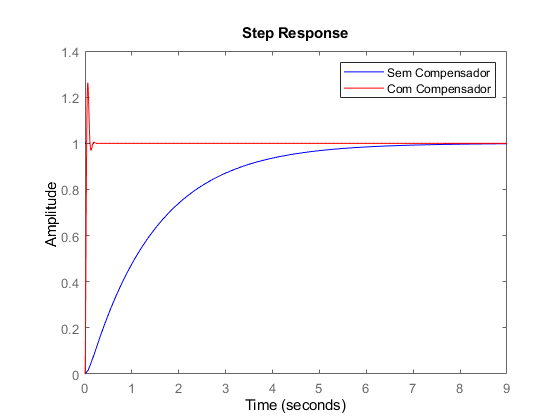
\includegraphics[width=0.85\textwidth]{images/fig5.png}
  \caption{Resposta ao degrau com e sem compensador}
\end{figure}

\begin{figure}[H]
  \centering
  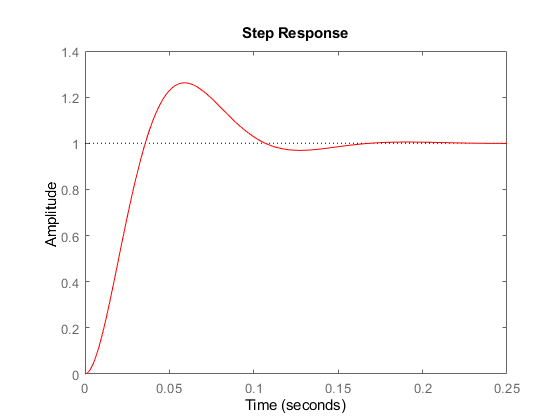
\includegraphics[width=0.85\textwidth]{images/fig6.png}
  \caption{Resposta ao degrau com compensador}
\end{figure} \newpage

%%%%%%%%%%%%%%%%%%%%%%%%%%%%%%
%             PARTE 8
%%%%%%%%%%%%%%%%%%%%%%%%%%%%%%

\noindent \textbf{7. Obter o erro estático e compará-lo com o erro estático especificado. .}\\

Para achar o valor do erro estático foi utilazado o matlab, foi encontrado o valor numérico e feito o gráfico comparando a resposta a rampa dos sistemas com e sem compensador, segue o código:

\begin{lstlisting}[style=matlab]
t=0:0.01:2;
Yg_R=feedback(G,1);
yg=lsim(Yg_R,t,t);

figure(6)
y=lsim(Y_R2,t,t);
figure(6)
plot(t,t,'k',t,y,t,yg);
xlabel('tempo')
ess=t(end)-y(end)
\end{lstlisting}\vspace{0.2cm}

O código resultou num erro estático igual a,

{\color{red} \[\boxed{e_{ss} = 0,0100}\]}

O que fechou exatamente com o valor específicado, vendo o gráfico:

\begin{figure}[H]
  \centering
  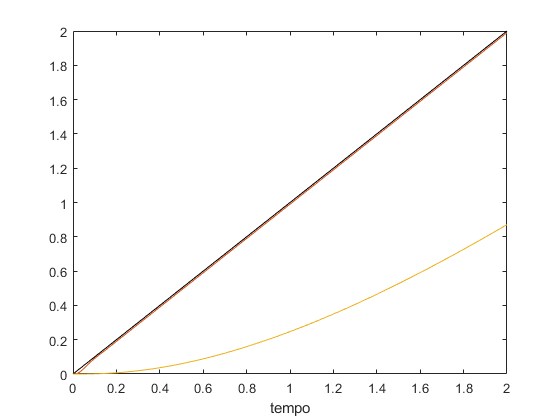
\includegraphics[width=0.85\textwidth]{images/fig7.png}
  \caption{Resposta a rampa com e sem compensador}
\end{figure}

Fica claro que o sistema compensado fica quase totalmente sobre a rampa. O que comprova mais ainda a assertividade do projeto. \newpage






























